\chapter{Hardware and Softwarestack}\label{ch:hardware-and-softwarestack}


\section{Overview}

The mobile application will be developed for Android and tested using a Google Pixel 7.
It will be coded in Kotlin using Android Studio.

The Google ARCore API will be used to access depth information about a scene.
The API is available by default -- no additional libraries are required.

Algorithms will be implemented in C\texttt{++} in the \texttt{procedural-augmented-reality} project provided by Prof. Dr. Phillipp Jenke.
The project will be embedded into the application and will be called through a binding layer from Kotlin.


\section{ARCore Depth API Hello World}

The \href{https://developers.google.com/ar/develop/java/depth/quickstart}{quickstart section} of the documentation of
the ARCore Depth API provides a sample application named \texttt{hello\_ar\_kotlin}.
The \texttt{hello\_ar\_kotlin} application has been confirmed to run on the hardware mentioned above.
Screenshots of the running application can be seen in figure~\ref{fig:hello_world_screenshot}.


\begin{figure}[ht!]
    \centering
    \begin{subfigure}[t]{.45\textwidth}
        \centering
        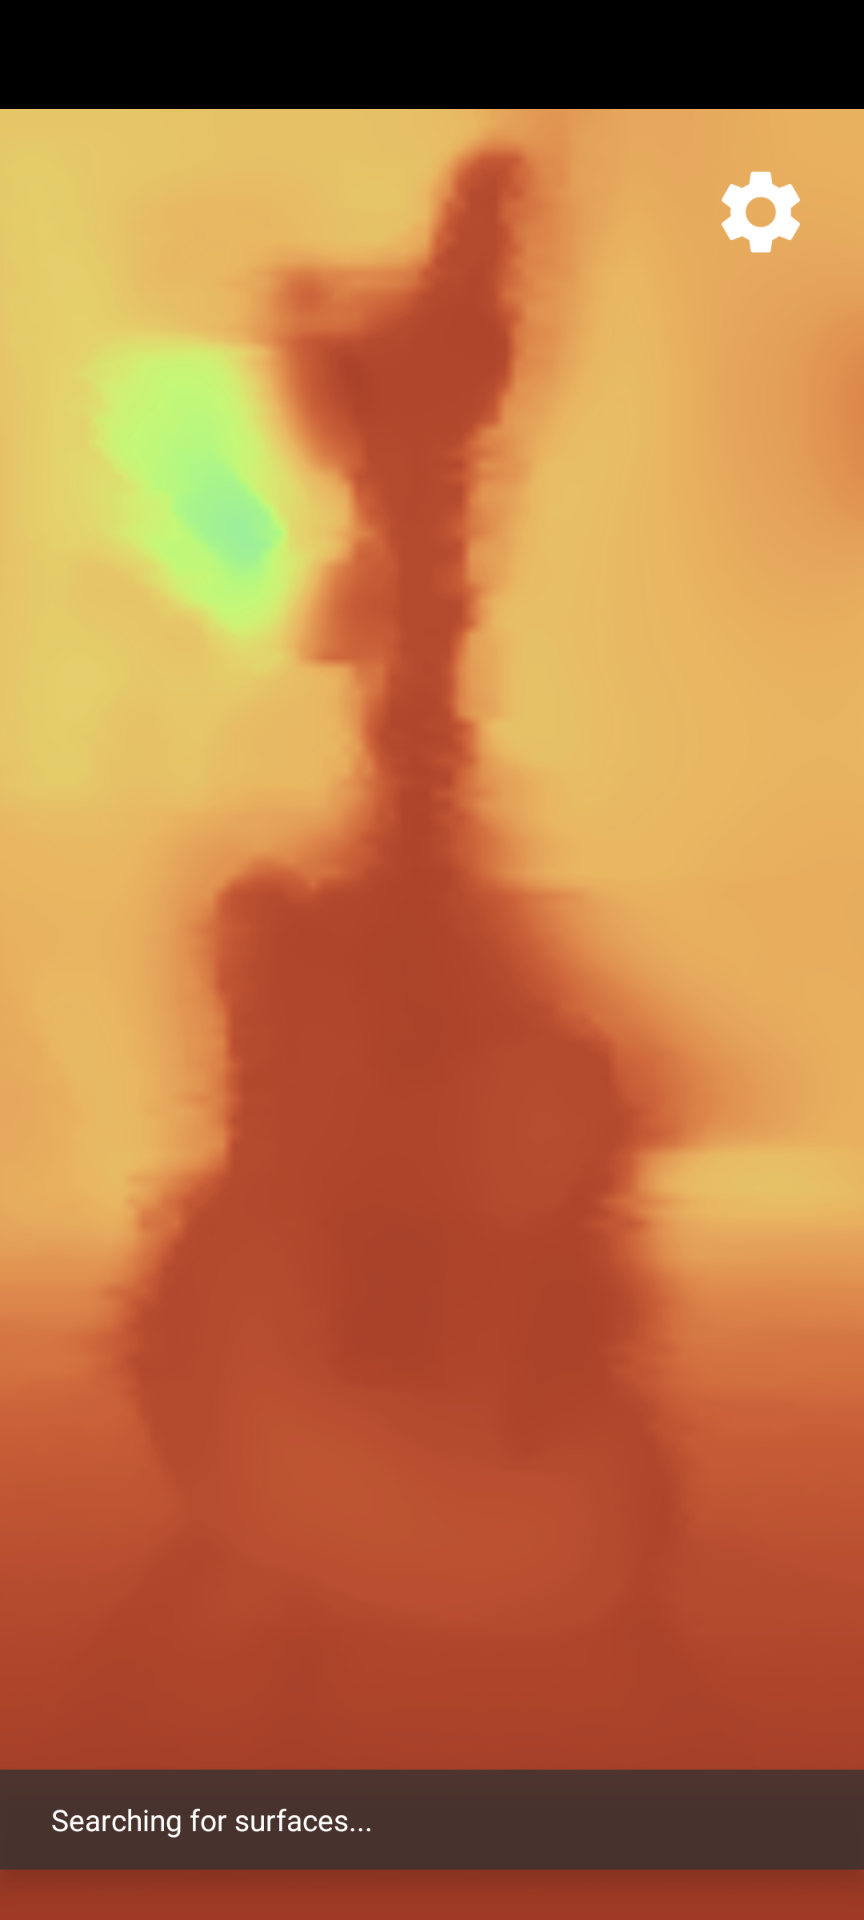
\includegraphics[width=.8\textwidth]{images/depth_api_hello_world_depth}
        \caption{Depth image, colors represent depth}
    \end{subfigure}\hfill
    \begin{subfigure}[t]{.45\textwidth}
        \centering
        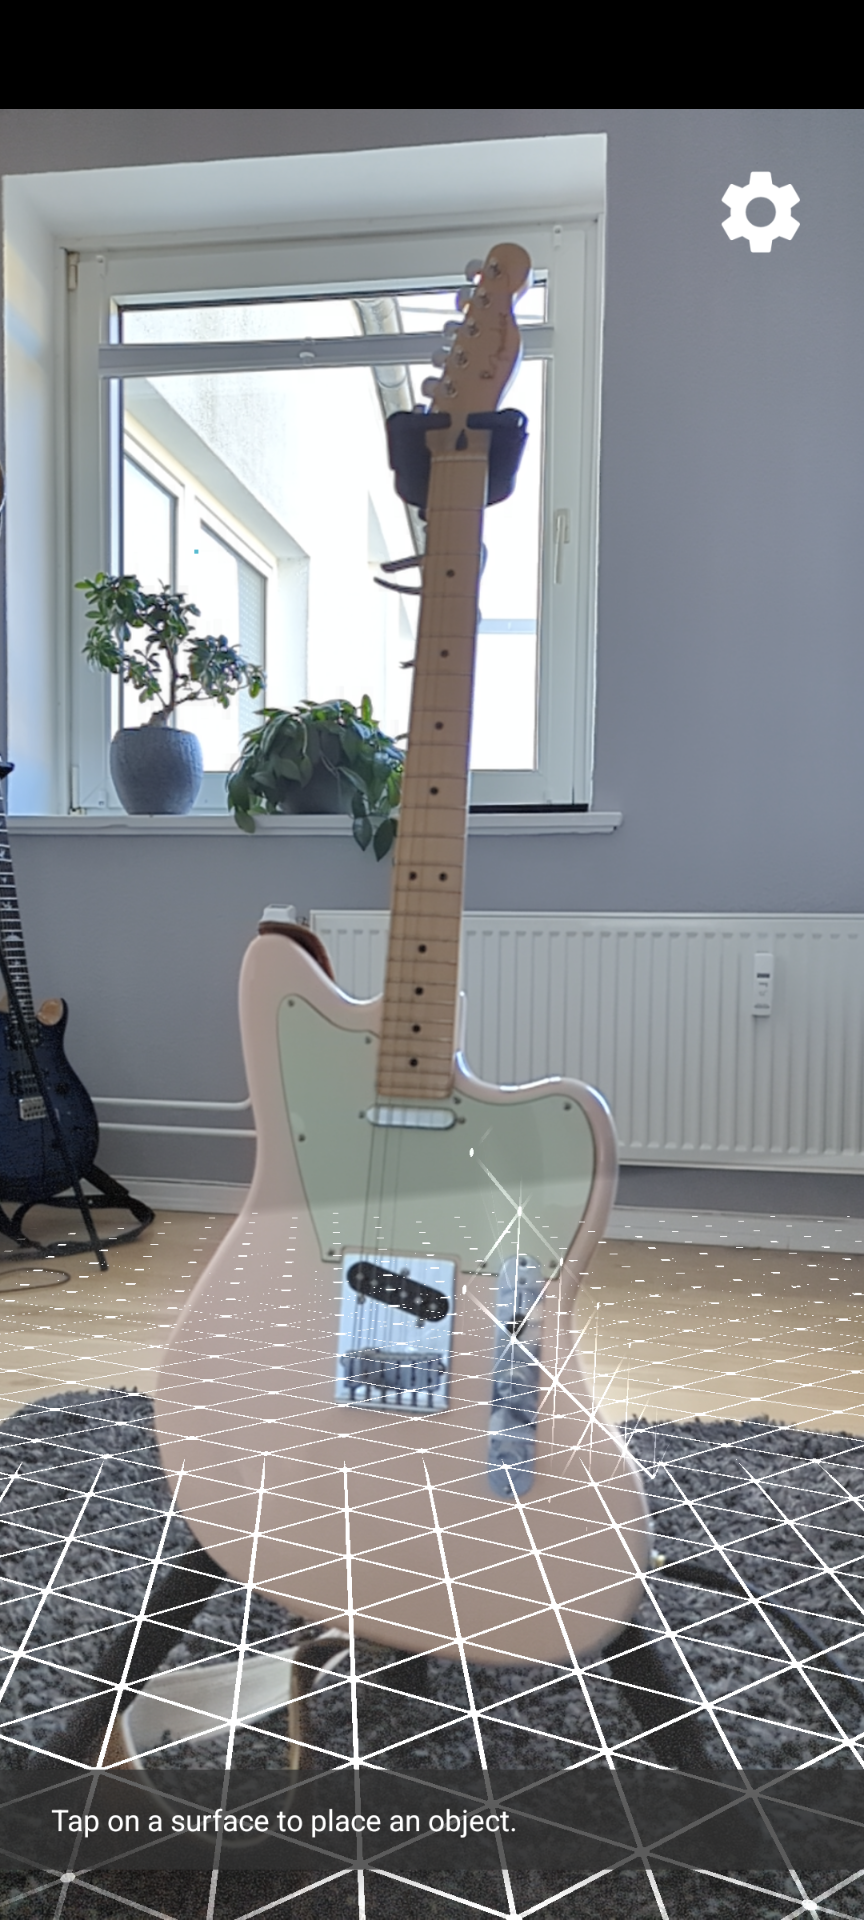
\includegraphics[width=.8\textwidth]{images/depth_api_hello_world_img}
        \caption{Full color reference}
    \end{subfigure}
    \caption{Screenshots of the \texttt{hello\_ar\_kotlin} application running on a Pixel 7}
    \label{fig:hello_world_screenshot}
\end{figure}
